\documentclass{article}
\usepackage{algorithmicx}
\usepackage{algpseudocode}
\usepackage{graphicx}
\usepackage{color}
\usepackage[utf8]{inputenc}

\begin{document}
{\noindent \Huge Problema a resolver:}
\newline \newline  El problema esta dado por la siguiente situaci\'on: 
tenemos en un $"$lista$"$ con una cantidad \textit{3$*$n} de n\'umeros(n un n\'umero fijo).\newline
Para \textit{i} desde \textit{0} a \textit{n-1}, vamos a decir la posici\'on \textit{i} en la lista va a ser \textit{Izq} del edificio \textit{i-\'esimo}, \textit{i+1} va a ser \textit{Alt} del edificio \textit{i-\'esimo} e \textit{i+2} va a ser \textit{Der} del edificio i-\'esimo.\newline
A grandes rasgos vamos a tener una lista de \textit{n} edificios (interpretamos a un edificio como una tupla \textit{$<$Izq,Alt,Der$>$}) con una base en com\'un impl\'icita que es 0.\newline
Por ejemplo para un entrada de la forma: \newline
\textit{n=3} y \textit{lista$=$ $<$1,2,3$>$,$<$4,2,7$>$,$<$2,4,6$>$} proyectada en un gr\'afico quedar\'ia:
\vspace{0.4cm}
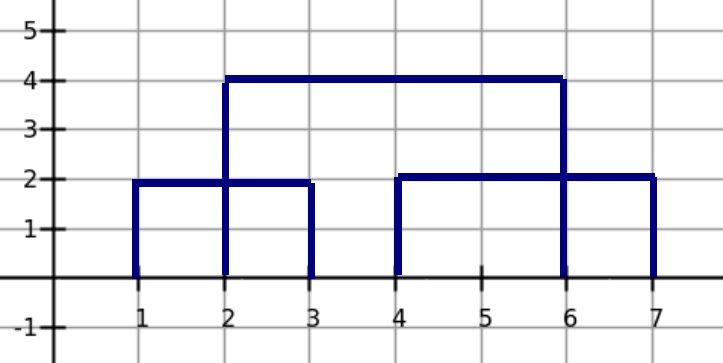
\includegraphics[width=\textwidth,height=\textheight,keepaspectratio
]{edificiosGraf1.png}
\begin {flushleft}
\end{flushleft}

Lo que queremos hacer es $"$eliminar todas las lineas interiores del gr\'afico$"$, quedarnos con su contorno, se obtiene el mismo resultado  "siguiendo con el dedo el gr\'afico". \newpage
Para una \textit{lista$=$ $<$0,3,8$>$,$<$1,6,5$>$,$<$2,4,6$>$,$<$4,2,7$>$,$<$9,6,10$>$} con \textit{n=5} su gr\'afico es: \newline
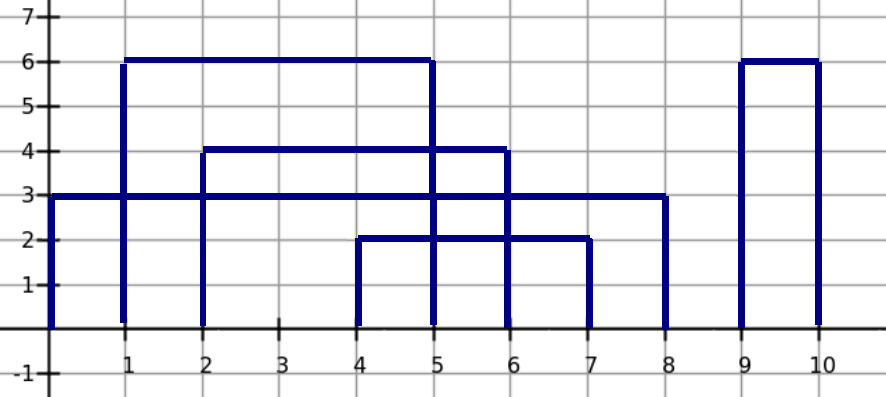
\includegraphics[width=\textwidth,height=\textheight,keepaspectratio
]{edificiosGraf2.png}
\begin {flushleft}
\end{flushleft}
el gr\'afico de eliminar las lineas interiores es:\newline
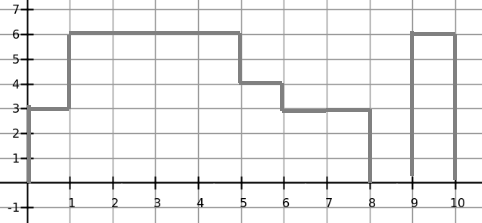
\includegraphics[width=\textwidth,height=\textheight,keepaspectratio
]{edificiosGraf2b.png}
\begin {flushleft}
\end{flushleft}
\newpage
El gr\'afico de "seguir con el dedo" es: \newline
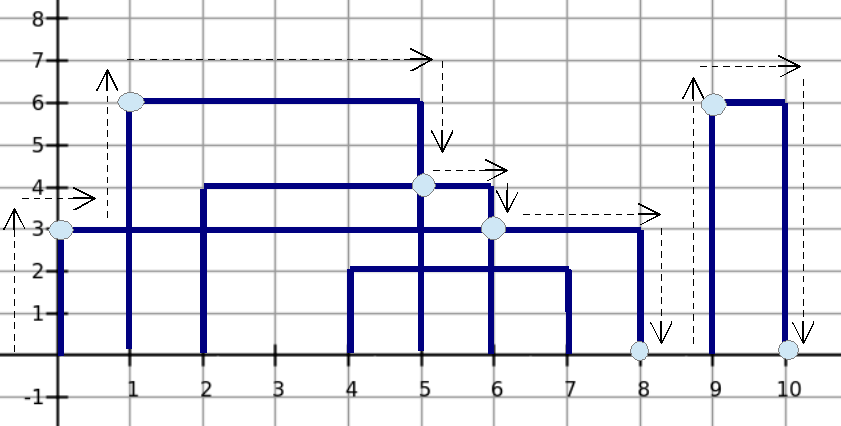
\includegraphics[width=\textwidth,height=\textheight,keepaspectratio
]{edificiosGraf2c.png}
\begin {flushleft}
La salida para este ejemplo es \textit{salida={0,3,1,6,5,4,6,3,8,0,9,6,0}}
\end{flushleft}

Lo que hago cuando "sigo con el dedo" es: \newline
Empezar con el primer edificio y seguimos el trazo, si me interseco con otro edificio seguir el trazo del edificio con el que me intersequ\'e desde ese punto. \newline
Si no me interseco con nadie pero hay m\'as edificios adelante "siguir con el dedo" los otros. Si no hay más edificios termin\'e.\newline
Luego de ese contorno voy a obtener la soluci\'on final que son los puntos donde hay cambios($\uparrow$ $\longrightarrow$ y $\downarrow$ $\longrightarrow$). \newline

\newpage

{\noindent \Huge Resoluci\'on:}
\newline \newline
Un panorama de la resolución es:\newline
ordenar los edificios por su Izq y retornar el primer punto del primer edifico. Vamos recorriendo los edificios(mirando el edificio por el que voy,anterior, y uno mas adelante,siguiente), si anterior interseca a siguiente, encolo anterior y retorno la intersección si siguiente es mayor en altura que anterior.\newline
Si es igual en altura o mayor, ahora anterior es siguiente. Si es menor en altura no hago nada. \color{red}{no vale la pena ponerlo} \newline \color{black}{}
Si anterior no interseca a siguiente(quiere decir que están "separados",pero puede que antes de anterior haya un edificio que termine despues que anterior y sea menor en altura )
voy a buscar este edificio en la cola (ordenada por altura) desencolando y mirando el tope:\newline
si lo encuentro, ese edificio ahora es anterior, retorno la intersección.\newline
si la cola es vacía(quiere decir que no había ningún edificio que terminara después que anterior) retorno anterior.Der,0,siguiente.Izq,siguiente.Alt y ahora anterior es siguiente.
\newline
Terminé de recorrer los edificios,pero puede que hayan quedado cosas dentro del heap, y son puntos que debería tener la solución
Mientras el heap tenga edificios, voy a comparar el tope con anterior:\newline
si tope termina antes que el anterior desencolo, en caso contrario imprimo la intersección. 
Ahora anterior es el toper de la cola y desencolo.
\newline
Hay cosas que en esta descripción no tuve en cuenta, porque son muy especificas en casos "borde", para explicarlo profundamente lo hago con este pseudocódigo: 
\newline
 
Sea lista: lista($<$Izq,Alt,Der$>$) y n la cantidad de tuplas en la lista.


\vspace{0.4cm}
\begin{algorithmic}[1]
\Procedure{ResolverEdificios}{$lista$,$n$}
	\State $ordenar los edificios por Izq$
	\State $comparo\gets lista[0]$
	\State $cola\gets vacio$
	\State $\textit{imprimo el primer punto}$
	\For{$(i\gets 1, n-1)$} \textit{$//$voy recorriendo los edificios}
		\State $siguiente\gets lista[i]$
		\If{$(\textit{se intersecan comparo y siguiente\color{red}{*0}})$}
			\If{$(\textit{siguiente $>$ comparo en altura \color{red}{*1}})$}
				\State $\textit{imprimir intersección}$
				\If{$(\textit{la cola está vacia})$}
					\State $\textit{cola.encolar(comparo)}$
				\Else
					\If{$(\textit{comparo no está en el tope del cola}$)}
					\State$\textit{cola.encolar(comparo)}$						
					\EndIf			
				\EndIf
					\State $comparo\gets siguiente$
			\EndIf
			\If{$(\textit{siguiente $==$ comparo en altura \color{red}{*2}})$}
				\If{$(\textit{la cola está vacia})$}
					\State $\textit{cola.encolar(comparo)}$
				\Else
					\If{$(\textit{comparo no está en el tope del cola}$)}
					\State$\textit{cola.encolar(comparo)}$
					\EndIf			
				\EndIf
			\EndIf
			\If{$(\textit{siguiente $<$ comparo en altura \color{red}{*3}})$}
				\State $cola.encolar(comparo)$
			\EndIf
			
		\EndIf \textit{(no se intersecan comparo y siguiente\color{red}{*4})}
		\If{$(\textit{la cola no está vacia})$}
			\While{$(\textit{cola no vacia})$}
				\If{$(\textit{primero.cola termina antes que siguiente \color{red}{*5}})$}		
				\State $\textit{desencolar.cola}$
				\Else \textit{(primero.cola termina despues que siguiente \color{red}{*6})}
				\State $\textit{imprimir interseccion entre comparo y primero.cola}$
				\EndIf
			\EndWhile
		\Else{\textit{ //no pasé a nadie que cortaría a comparo, como no se intersecan imprimo ambos puntos}}
		\State $\textit{imprimir comparo.Der y 0 }$
		\State $\textit{imprimir siguiente.Izq y siguiente.Alt}$
		\State $comparo\gets siguiente$
		\EndIf
	\EndFor{\textit{(no hay siguiente,puede que hayan quedado cosas en el cola \color{red}{*7}})}
	\textit{//uso a comparo que es el último edificio con el que haya en el tope de la cola}
	\While{$(\textit{la cola no sea vacia})$}
	\If{$(\textit{comparo termina antes que primero.cola \color{red}{*8})}$}
		\State $\textit{imprimir intersección comparo y primero.cola}$
		\State $comparo\gets cola.primero$
		\State $desencolar.cola$
	\Else{\textit{(comparo termina después que el primero.cola \color{red}{*9})}}
	\State $\textit{desencolar.cola}$
	\EndIf
	\EndWhile{(\textit{al último punto no lo imprimo nunca\color{red}{*9})}}\newline
	\textit{$//$lo imprimo acá}
	\State $\textit{imprimir comparo.Der y 0}$
\EndProcedure
\end{algorithmic}

\newpage

{\noindent \Huge Complejidad:}
\newline \newline
Vamos a ver que la cantidad de veces que encolo es una funcion de n, y así poder ver que la cantidad de veces que desencolo es tambien una funcion de n porque no puedo desencolar más cosas de las que encolo.
Vemos en el algoritmo que en el if *1 y *2,encola si está vacia y si el elemento está en el tope no lo encolo,(\color{red}{falta demostrar que si quiero encolar un elemento 2 veces el que quiero encolar de nuevo está en el tope, la idea la había sacado angel})\color{black} en el if *3 encolo.
\newline
Como vamos recorriendo los edificios linealmente y encolo en consecuencia de lo dicho arriba la cantidad de veces que encolo es una funcion de n, más precisamente n.

Veamos ahora la complejidad del while dentro del for, en peor caso por casa edificio desencolo todos los edificios eso da una complejidad n*n, pero si analizamos más finamente, nunca podría para cada paso desencolar todos los edificios.\newline
Si voy por el edificio \textit{i} (\textit{i} entre \textit{0} y \textit{n-1}), tengo en el heap en peor caso \textit{i-1} edificios, entro en el while y desencolo \textit{i-1} edificios, sigo avanzando y llego a un edificio \textit{j} (\textit{j} entre \textit{0} y \textit{n-1} y es mayor que \textit{i}) ahora en el heap en peor caso tengo \textit{j-i} edificios, entro en el while y desencolo en peor caso \textit{j-i} edificios.
llego al último edificio \textit{n-1} y en peor caso tengo \textit{n-1- j} edificios en el heap, entro al while y desencolo \textit{n-1-j} veces.
Si sumo la cantidad de veces que hice desencolar en el recorrido lineal es n(suma de los intervalos).
Entonces hago n veces desencolar

Relacionando la parte de encolar y desencolar en el for
por cada edificio hago un encolar y una cantidad x de desencolar + c operaciones que tienen costo 1
Por lo visto anteriormente la suma de esos x es n, entonces el costo es  n*(costo de desencolar)+ n*(costo de desencolar) +c(constante \color{red}{**})\color{black}
\newline\
Solo nos falta analizar el while después del for, por lo visto anteriormente la cantidad que puede tener el heap es n, y hastas que se vacia hace n*(costo de desencolar)
En la implementación usamos una priority-queue como cola, el costo de encolar(push) es log(n),desencolar(pop) es log(n) y tope(top) es 1.
\newline
Al princio del algoritmo ordeno los edificios por Izq, el costo de ordenarlos es n*log(n) (porque uso sort de la stl \color{red}{según este link} \color{black}), primero hago un swap de Alt por Izq(porque $<$ está definido por la posición Alt en la tupla) luego uso sort y por último vuelvo las posiciones de las tuplas a como estaban anteriormente.\newline
Entonces hago n[\textit{de invertir tuplas} + n*log(n)[\textit{de ordenarlos} + n[\textit{invertira las tuplas de nuevo} 

Finalmente la complejidad es O(n[\textit{de invertir tuplas}] + n*log(n)[\textit{de ordenarlos}] + n[\textit{invertir las tuplas de nuevo}] + c[\textit{operaciones}]+n[\textit{encolar}]+n*(log(n))[\textit{desencolar del for}] + n*log(n)[\textit{desencolar del while después del for}]) $\in$ O(n(log(n))) \newline
\color{red}{**} \color{black}
\newpage



{\noindent \Huge Correctitud:}
\newline \newline
El algoritmo pone el primer punto y el último SIEMPRE.(dónde lo hace!!!)
Quiero ver que va a poner los puntos intermedios correctamente
Tengo los edificios ordenados por izquierda y accedo a ellos secuencialmente mirando el edificio por el que voy(anterior) y el siguiente:

Si anterior y siguiente se intersecan:\newline
	si anterior es mayor a siguiente (grafico A)\newline
		tengo que poner el punto de intersección en la solución\newline
		Supongamos que ese punto (intersección) no es solución:\newline
			caso (gráfico B) existe un edificio que empieza entre ia y is, termina después que is y tiene altura entre as y aa :\newline
			si existiera este edificio tendría que se siguiente , ABS!!!\newline
			Entonces el punto es solución.\newline
			caso (grafico C) exite un edificio que empieza antes que ia, tiene altura mayor aa y termina después que is:\newline
			Si existiera tendría que se anterior , ABS!!!\newline
			Entonces el punto es soución.\newline

Si no se intersecan anterior y siguiente():\newline
	voy a tener en el heap los edificios que terminan después que empieza el anterior porque los fui enconlando (grafico D)
	si el heap está vacío quiere decir que no hay nadie que corte a anterior. \newline
		Entonces voy poner en la solución el punto de anterior y el punto de siguiente.\newline
	Si el heap no está vacío quiere decir que puede que tenga un edificio que corte a anterior 
		voy a sacar del heap hasta que encuentro uno que interseque a anterior, por como es el heap (está ordenado por mayor altura) este que me interseca es el que tiene mayor altura, entonces este punto
		de intersección es solución.\newline
		Supongamos que este punto de intersección no es solución.\newline
		caso (grafico E) exite un edificio que empieza antes que d, termina despues que ad y tiene altura entre aa y ha, entonces este si exitiera, lo tendría que haber encolado cuando reccorría los edificios y tendría que ser el edificio que me daría el heap ABS!!!\newline
		Entonces es solución.\newline

\end{document}